\documentclass[twoside]{report}

\usepackage[landscape,inner=2cm,outer=12cm,marginparwidth=9cm,
            marginparsep=1.0cm,bottom=2cm]{geometry}

\setlength{\parskip}{1.1em}
\setlength{\parindent}{0em}
\usepackage{pdfpages}
\usepackage{amsmath}
\usepackage{amsfonts}
\usepackage{amssymb}
\usepackage{bigdelim}
\usepackage[usenames,dvipsnames]{pstricks}
\usepackage{booktabs}
\usepackage[T1]{fontenc}
\usepackage{listings}
\usepackage[T1]{fontenc}
\usepackage[utf8]{inputenc}
\usepackage{float}
\usepackage{graphicx}
\usepackage{cite}
\usepackage{hyperref}
\usepackage{layout}
\usepackage{titlesec}
\usepackage{fancyhdr}
\usepackage{pgf}
\usepackage{amsmath}
\usepackage{titlesec}
\usepackage{verbatim}
\usepackage{color}
\usepackage[font=small,labelfont=bf]{caption}
\usepackage{marginnote}
\usepackage{afterpage}
\usepackage[default,light]{roboto}
\usepackage{sectsty}


\usepackage{tikz}
\usepackage{circuitikz}

% No number sections
\renewcommand{\thesection}{}
\renewcommand{\thesubsection}{\arabic{section}.\arabic{subsection}}
\makeatletter
\def\@seccntformat#1{\csname #1ignore\expandafter\endcsname\csname the#1\endcsname\quad}
\let\sectionignore\@gobbletwo
\let\latex@numberline\numberline
\def\numberline#1{\if\relax#1\relax\else\latex@numberline{#1}\fi}
\makeatother

%Colors
\definecolor{front}{RGB}{246, 104, 0}
\definecolor{sec}{RGB}{246, 104, 0}


% Paragraphs have proper breaks
\titlespacing\section{0pt}{12pt plus 4pt minus 2pt}{0pt plus 2pt minus 2pt}
\titlespacing\subsection{0pt}{12pt plus 4pt minus 2pt}{0pt plus 2pt minus 2pt}
\titlespacing\subsubsection{0pt}{12pt plus 4pt minus 2pt}{0pt plus 2pt minus 2pt}
\renewcommand{\figurename}{{\textbf{Image}}}
\sectionfont{\color{front}}

%Fancyheader
\pagestyle{fancy}
\fancyheadoffset[leh,roh]{10cm}
\fancyhf{}
\fancyhead[LE,RO]{\textcolor{gray}{\thepage \quad | \quad \textsc{Pilot Study}}}
\fancyhead[RE,LO]{\textcolor{gray}{}}
\renewcommand{\headrulewidth}{0pt}

%Define commands
\newcommand{\marginquote}[1]{\marginpar{\textcolor{gray}{\large\itshape\fontfamily{ppl}\selectfont``#1''}}}

\begin{document}
\begin{titlepage}
  %\vspace{12cm}
	\raggedright
  {\Large{\colorbox{front}{\color{white} \textbf{PROJECT NAME}\kern 1pc}}\\\vspace{0.3cm}}
  {Pilot Study\\}
  \vfill
	{\large \today\par}
  {\small\color{gray} Marc Coquand, Linus Lagerhjelm, Mattias Cederberg and Simon
  Asp\\}
  {\small\color{gray} Supervised by Stig Byström}\\
  {\small\color{gray} Umeå University\\}

	%\vfill

\end{titlepage}

\renewcommand{\baselinestretch}{1.0}

\newpage

\pagecolor{front}\afterpage{\nopagecolor}\thispagestyle{empty}

\marginpar{\textcolor{white}{\small{Project
Management}\vspace{11cm}\\\large\textbf{Background}\\ {\small 
Walking home late at night can be a daunting experience. The newspapers write
about assaults and harassment, the northern winter climate contribute with
shorter days and darker nights. Existing street lights helps with the problem
but the feeling of uncertainty and fear persist. $PROJECTNAME$ will investigate
how a technical solution could be applied to create an increased sense of
safety. The project is carried out in collaboration with the municipality of
Umeå and Umeå University as part of the courses Interactivity in Smart
Environments and Project Management.
 }}} \newpage

\tableofcontents
\thispagestyle{empty}
\newpage

\section{Background}

Walking home late at night can be a daunting experience. The newspapers write
about assaults and harassment, the northern winter climate contribute with
shorter days and darker nights. Existing street lights helps with the problem
but the feeling of uncertainty and fear persist. $PROJECTNAME$ will investigate
how a technical solution could be applied to create an increased sense of
safety. The project is carried out in collaboration with the municipality of
Umeå and Umeå University as part of the courses Interactivity in Smart
Environments and Project Management

\section{Limitations}

\section{Specification Requirement}

\section{Analysis}

\section{The Team}
%\marginpar{ \captionof{figure}{This is a margin figure.}
%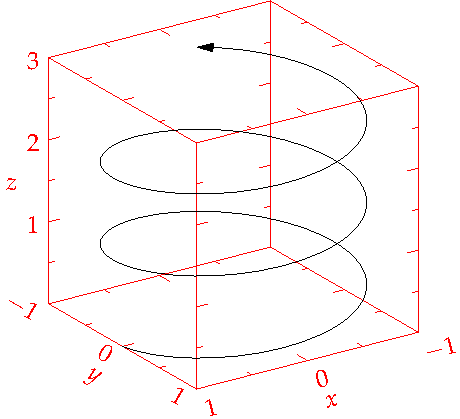
\includegraphics[width=\marginparwidth]{graphics/helix.pdf}} 

%\marginquote{This is a very insipirational quote right here. Very
%quoteworthy if I may say so myself.}

\end{document}
